\section{Geometria modelu ramena}
Na Obr. \ref{fig:geometria_ramena} je nákres schematického zobrazenia rozmerov robotického ramena.
\begin{figure}[h]
\centering
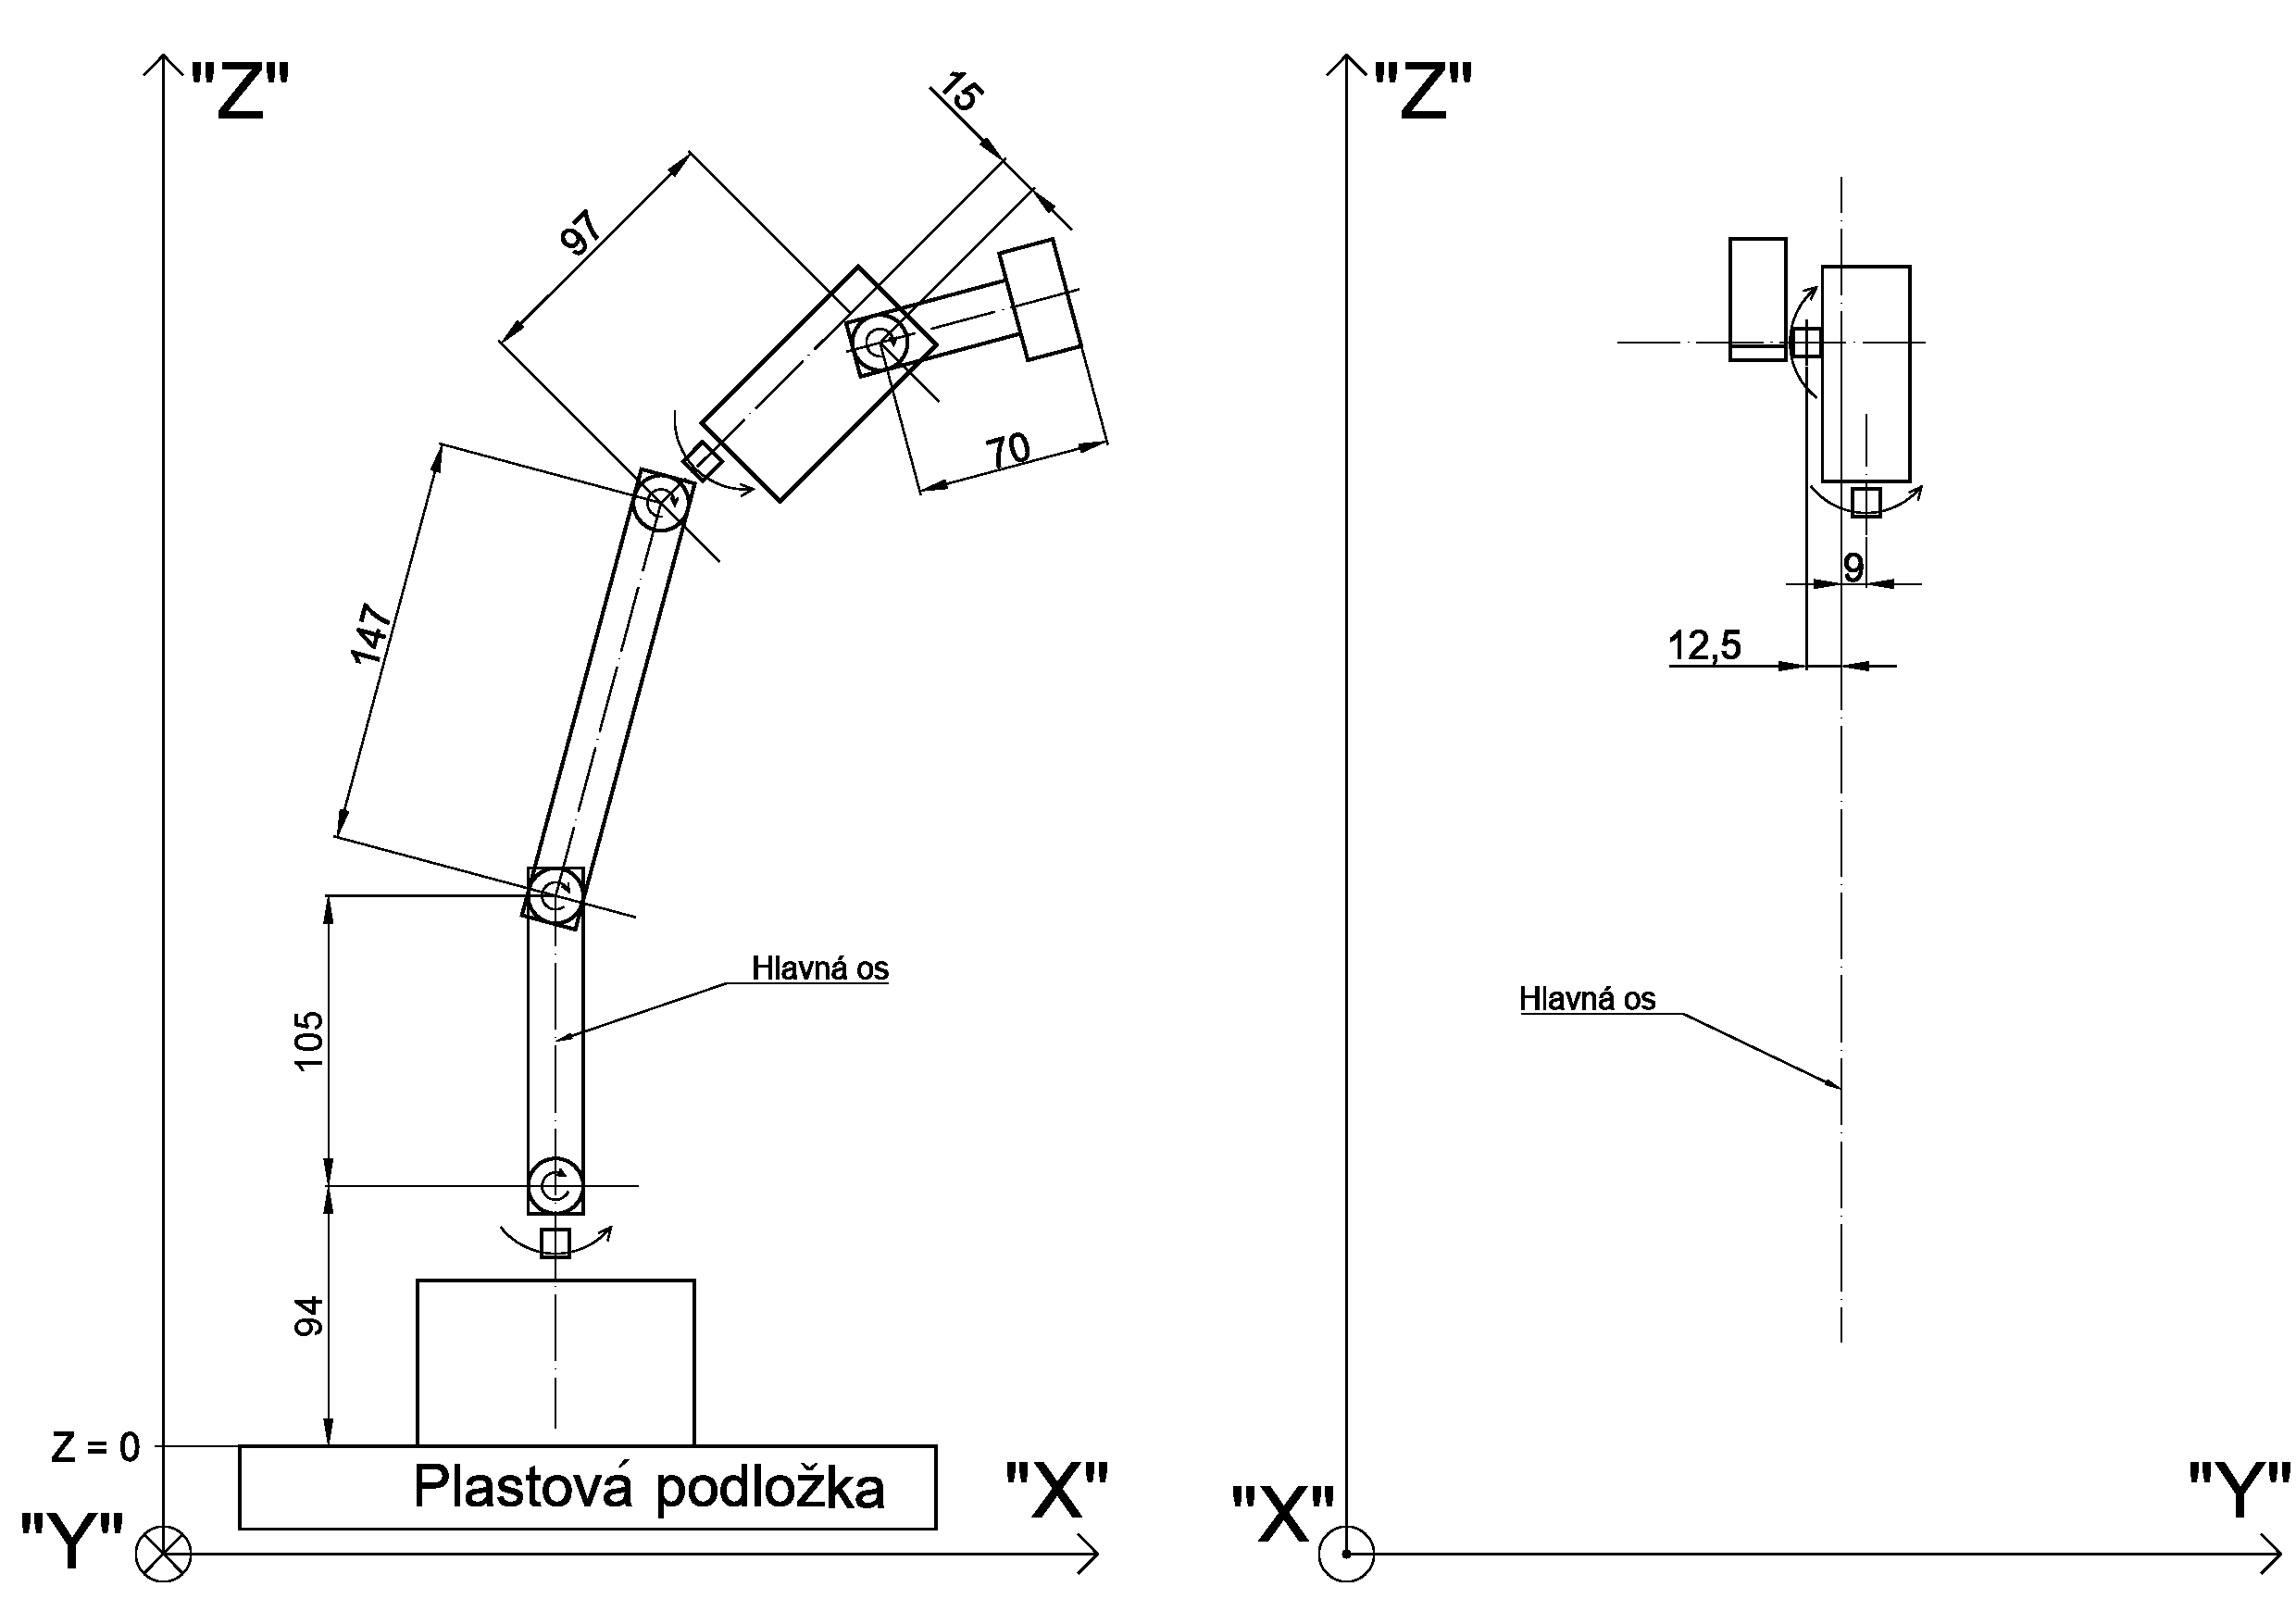
\includegraphics[width=0.8\textwidth]{img/TIM-PR_rameno_vykres.pdf}
\caption{Schematické zobrazenie rozmerov robotického ramena}
\label{fig:geometria_ramena}
\end{figure}

Rozmery posunutí rotácie bolo kvôli implementácii výpočtov pre inverznú kinematiku nevyhnutné správne určiť. 
Na ľavej časti nákresu je rameno zobrazené „z boku“, a teda os robota X smeruje vpravo a Y smerom do obrázka.
V pravej časti je zobrazenie ramena „spredu“, čiže os X smeruje von z obrázka a os Y smeruje vpravo.
Tým, že tieto nákresy slúžia len na zdokumentovanie posunutí kĺbov (bodov otáčania) ramena, 
nie sú zahrnuté celkové rozmery súčiastok ramena. Taktiež v pravej časti nákresu nie sú zobrazené 
prvé dva články ramena, lebo nemalo význam ich kresliť, keďže neboli v osi Y posunuté.
Čiarkovaná čiara oznažená ako hlavná os značí smer osi Z ramena.
Taktiež značí stred symetrie niektorých článkov robotického ramena, 
čo bolo vhodné využiť pri označovaní dĺžok posunutí kĺbov.
Kruhy so šípkou na koncoch článkov ramena označujú kĺby realizujúce rotáciu v osi Y a 
štvorce so šípkou označujú kĺby konajúce rotáciu v osi Z, prípadne kĺby realizujúce rotáciu v osi Y v inom pohľade.
Označenia osí v nákresoch, ktoré v úvodzovkách neoznačujú reálne osi X, Y a Z, 
resp. reálny stred súradnicového systému, ale slúžia len ako pomocné osi pre lepšiu vizualizáciu smeru,
z ktorého je nákres ramena realizovaný. Skútočný počiatok súradníc robotického ramena je v bod,
 kde sa pretína os označená „Z = 0“ a hlavná os.